\chapter{Sistema di autenticazione}
Il meccanismo di autenticazione è la procedura per verificare che un determinato dispositivo
è abilitato a connettersi alla rete.
Questo procedimento avviene tramite il riconoscimento dell'identificativo del cellulare (IMSI) e Successivamente
avviene l'\textit{Authentication and key agreement} (AKA), procedimento in cui
il \textit{core network} abilita un dispositivo a connettersi.\\
In questo capitolo verranno trattati le procedure di autenticazione\cite{identifications} per le generazioni dal 2G al 5G, il 1G è stato escluso 
poiché ha un funzionamento completamente analogico.

\clearpage

\section{2G}
Il sistema di autenticazione di seconda generazione utilizza principalmente due codici univoci della SIM e del MS:
\begin{itemize}
    \item IMSI ovvero un codice identificatvo della SIM
    \item IMEI ovvero un codice identificativo del MS
\end{itemize}
Questi due codici saranno necessari anche per le prossime generazioni fino al 4G.\\
La procedura di autenticazione di un MS segue questi passaggi:
\begin{enumerate}
    \item Il MS invia l'IMSI alla BTS di riferimento che lo inoltra al \textit{Core Network}, questo
    avviene ogni volta che il MS vuole connettersi al \textit{network} e non risulta già risultato presso 
    la rete di riferimento. In caso lo fosse, verrà utilizzato il TMSI \textit{Temporary MobileSubscriber Identity}
    per preservare il suo anonimato.
    \item L'AuC cerca la chiave Ki associata all'IMSI e insieme a un numero casuale RAND genera un codice SRES che verrà
    salvato nel VLR.
    \item Viene inviato al MS il RAND generato.
    \item La stessa procedura viene fatta dal MS, che genera quindi il suo SRES e lo invia al VLR
    \item Il VLR confronta se l'SRES ricevuto corrisponde a quello generato dall'AuC, se corrispondono l'autenticazione risulta
    effettuata con successo e viene generato,salvato e inviato il TMSI.
\end{enumerate}

\begin{figure}[h]
    \centering
    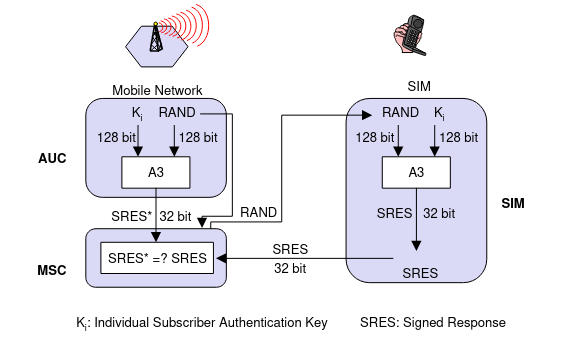
\includegraphics[width=0.7\textwidth]{images/auth-2g.png}
    \caption{Autenticazione nelle reti 2G}
\end{figure}

\clearpage

\section{3G-4G}
L'autenticazione nell'architettura di terza generazione è molto simile a quella della seconda salvo i seguenti miglioramenti:
\begin{itemize}
    \item Viene introdotta l'autenticazione mutua per prevenire l'autenticazione a false \textit{Base stations}.
    \item La lunghezza della chiave Ki viene incrementata da 64 a 128 bit.
    \item Viene implementato un flag per verificare se le comunicazioni vengono compromesse durante la trasmissione chiamato \textit{Integrity Key} (IK).
\end{itemize}
Il procedimento di autenticazione è il seguente\cite{4g-auth}:
\begin{enumerate}
    \item Il MS invia l'IMSI alla BTS di riferimento che lo inoltra al \textit{Core Network}
    \item L'AuC cerca la chiave Ki associata all'IMSI e insieme a un numero casuale RAND genera un codice SRES che verrà
    salvato nel VLR.
    \item VIene trovata la chiave Ki corrispondente all'IMSI dall'AuC, dopodichè viene generato un codice SRES con l'utilizzo di un numero randomico RAND.
    Inoltre, viene generato un codice AUTN per permettere al MS di autenticare il \textit{network}.
    \item Viene inviato al MS il RAND e AUTN.
    \item Il MS autentica il \textit{network} confrontando il valore di AUTN ricevuto. Se il \textit{network} è valido, prosegue con la generazione del SRES.
    \item Il VLR confronta se l'SRES ricevuto corrisponde a quello generato dall'AuC, se corrispondono l'autenticazione risulta
    effettuata con successo e viene generato,salvato e inviato il TMSI.
\end{enumerate}
\begin{figure}[h]
    \centering
    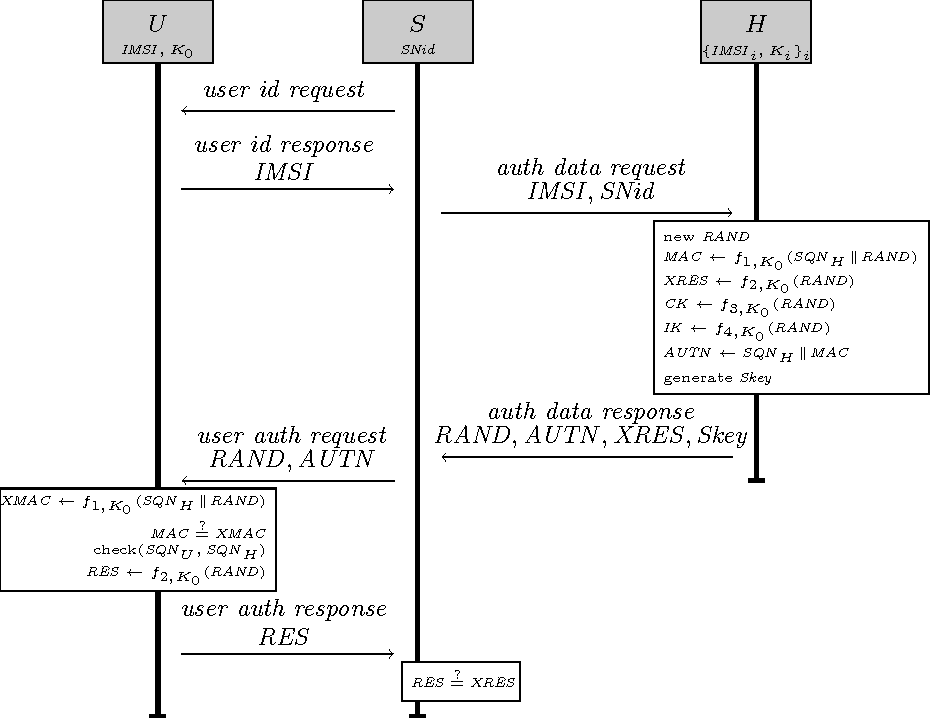
\includegraphics[width=0.7\textwidth]{images/auth-3g.png}
    \caption{Autenticazione nelle reti 3G}
\end{figure}

\clearpage

\section{5G}
L'autenticazione della generazione 5G è molto diversa dalle precedenti poichè, come illustrato nella sezione (?), l'architettura è completamente rivista diventando una ramificazione di microservizi.
Sono definiti tre protocolli di autenticazione:
\begin{itemize}
    \item 5G-AKA: 5G-Authentication and Key Management
    \item EAP-AKA: Extensible Authentication Protocol – Authentication and Key Management
    \item EAP-TLS: Extensible Authentication Protocol – Transport Layer Security
\end{itemize}
Rispetto alle generazioni precedenti ci sono stati i seguenti miglioramenti di sicurezza\cite{5g-vs-4g}:
\begin{itemize}
    \item L'IMSI non viene mai comunicato in chiaro ma sempre criptato
    \item I componenti del \textit{network} coinvolti sono dei servizi
\end{itemize}
L'autenticazione è fondamentalmente diviso in due parti: La prima è l'inizializzazione dell'autenticazione e la scelta del metodo di autenticazione.
La seconda è invece l'autenticazione mutua come avviene nelle generazioni precedenti.
Lo schema di autenticazione è il seguente\cite{5g-auth}:
\begin{enumerate}
    \item Il MS invia il SUCI o 5G-GUTI alla BTS di riferimento che lo inoltra al AMF/SEAF
    il GUTI è un identificativo temporaneo simile al TMSI delle generazioni precedenti, invece il SUCI è un identificatore criptato
    permanente.
    \item il SEAF manda l'identificatore del dispositivo (SUCI o 5G-GUTI) e il \textit{Serving Network Name} (SNN) all'AUSF.
    Il SNN è una concatenazione di codici identificativi di servizi e il codice identificativo del \textit{Serving Network}.
    \item L'AUSF controlla che la richiesta dal SEAF sia autorizzata a utilizzare il SNN, in caso non lo fosse risponde con un 
    apposito messaggio di errore.
    \item L'AUSF reperisce la chiave associata all'identificativo nell'archivio UDM e genera il rispettivo SRES con un numero randomico RAND.
    \item Viene inviato all'MS il RAND e AUTN (per l'autenticazione mutua).
    \item Il MS procede con la creazione del SRES e lo invia al SEAF.
    \item Il SEAF inoltra il SERS all'AUSF che si occupa di controllare se corrispondono e in caso confermare l'autenticazione.
\end{enumerate}
\begin{figure}[h]
    \centering
    \includegraphics[width=0.8\textwidth]{images/auth-5g.png}
    \caption{Autenticazione nelle reti 5G}
\end{figure}